\section{Numerical Experiments}\label{sec:experiments}
\subsection{Convergence tests}
We verified the implementation of the forces by performing a convergence test of a first order finite difference approximation. Let $e_\alpha$, $\alpha=1,2,3$, be the canonical unit vectors of $\mathbb R^3$, and define the forward finite difference
\[
	F_{i,\alpha}(\delta)
	= 
	\frac{E_s(x_1,\ldots,x_i + \delta e_\alpha,\ldots,x_M) - E_s(x_1,\ldots,x_i,\ldots,x_M)}{\delta}
\]
where we have made explicit the dependency of the solvation energy on the nuclear positions $x_1 , \ldots , x_M$. It immediately follows that $\mathcal{F}_{i,\alpha} = F_{i,\alpha}(\delta) + O(\delta)$, where $\mathcal{F}_{i,\alpha}$ is the $\alpha$ component of $\mathcal{F}_i$, which implies that the relative error $\text{Err}_{i,\alpha}(\delta) = |(\mathcal{F}_{i,\alpha} - F_{i,\alpha}(\delta))/\mathcal{F}_{i,\alpha}|$ decreases as $O(\delta)$, namely with rate 1.

We investigated the rate of convergence for a molecular configuration composed of six spheres with radius 1.5 and centers at $x_{\pm \alpha} = \pm e_\alpha$, for $\alpha = 1, 2,3$. Although conceptually simple, this configuration generates a sextuple intersection which provides a challenging benchmark case. We have studied the behavior of the relative error over the range of angular momenta $\ell = 2, \ldots , 10$, and obtained numerical results that are qualitatively similar, and in excellent agreement with the predicted rate of convergence. Results for a representative case are reported in Table \ref{tab:1}.

%\begin{tabular}{ l l l l}
%\toprule
%Expression & \ multicolumn {1}{ c }{ Value } \\ %\otoprule
%$\pi $ & 3 ,1416 \\ \midrule
%$\pi ^{\pi }$ & 36 ,46 \\ \midrule
%$\pi ^{\pi ^{\pi }}$ & 80662 ,7 \\ \bottomrule
%\end{tabular}

\begin{table}[t]
\footnotesize
\begin{center}
	\begin{tabular}{ @{}cccc  cccc  cccc @{} }
\toprule[0.1em] 
\multirow{2}{*}{\bf Derivative} & $\phantom{abs}$ &  \multicolumn{1}{c}{$\delta = \delta_0$}& $\phantom{abs}$  & \multicolumn{2}{c}{$\delta = \delta_0/2$}& $\phantom{abs}$  & \multicolumn{2}{c}{$\delta = \delta_0/4$}& $\phantom{abs}$  & \multicolumn{2}{c}{$\delta = \delta_0/8$} \\
		         \cmidrule[0.05em]{3-3}  \cmidrule[0.05em](lr){5-6}  \cmidrule[0.05em]{8-9}   \cmidrule[0.05em]{11-12}
&	& {\sl Error}	&& {\sl Error}	& {\sl Rate} && {\sl Error}	& {\sl Rate}&& {\sl Error}	& {\sl Rate} \\
%			 & $\delta = \delta_0/2$& $\delta = \delta_0/4$& $\delta = \delta_0/8$ \\
\midrule[0.05em]
$x_{+1,1}$ &  &  0.23529E-02  &  &    0.11751E-02  &  1.002  &&  0.58717E-03  &  1.001  &&  0.29345E-03  &  1.001  \\
$x_ {-1,1}$  &&  0.23529E-02  &   &  0.11751E-02  &  1.002  &&  0.58718E-03  &  1.001  &&  0.29344E-03  &  1.001  \\
$x_ {+2,2}$  &&  0.23529E-02  &   & 0.11751E-02  &  1.002  &&  0.58692E-03  &  1.002  &&  0.29411E-03  &  0.997  \\
$x_ {-2,2}$  &&  0.23529E-02  &    &0.11751E-02  &  1.002  &&  0.58719E-03  &  1.001  &&  0.29348E-03  &  1.001  \\
$x_ {+3,3}$  &&  0.23529E-02  &  &  0.11751E-02  &  1.002  &&  0.58718E-03  &  1.001  &&  0.29344E-03  &  1.001  \\
$x_ {-3,3}$  &&  0.23529E-02  &   &  0.11751E-02  &  1.002  &&  0.58720E-03  &  1.001  &&  0.29337E-03  &  1.001  \\
\bottomrule[0.1em]
\end{tabular}
\caption{Relative error and converge rate for a configuration of 6 spheres with radii equal to 1.5, and centers $x_{\pm \alpha} =  \pm e_\alpha$ for $\alpha = 1, 2,3$.  Results where obtained with an angular momentum $L_\text{max} =  8$, and an integration grid with $N_\text{grid} = 110$ nodes. Each atomic position coordinate $x_{\pm\alpha,\beta}$, where $\beta = 1,2,3$, was perturbed as $(1 + \delta)x_{\pm\alpha , \beta}$, thus generating only six nonzero variations, starting from an initial value $\delta_0 = 10^{-3}$.}\label{tab:1}
\end{center}
\end{table}
These results prove the correctness of our implemetation. 
% lmax =  8 , ngrid =  110 - Integration points PRESENT in the switch region
% eta = 0.2, s = 0
% delta = 10^-3
% Relative error : 
% dE / dr_ 1,1 :  0.23529E-02   0.11751E-02   0.58717E-03   0.29345E-03
% dE / dr_ 2,1 :  0.23529E-02   0.11751E-02   0.58718E-03   0.29344E-03
% dE / dr_ 3,2 :  0.23529E-02   0.11751E-02   0.58692E-03   0.29411E-03
% dE / dr_ 4,2 :  0.23529E-02   0.11751E-02   0.58719E-03   0.29348E-03
% dE / dr_ 5,3 :  0.23529E-02   0.11751E-02   0.58718E-03   0.29344E-03
% dE / dr_ 6,3 :  0.23529E-02   0.11751E-02   0.58720E-03   0.29337E-03
% 
% Rate of convergence : 
% dE / dr_ 1,1 :        0.000        -1.002        -1.001        -1.001
% dE / dr_ 2,1 :        0.000        -1.002        -1.001        -1.001
% dE / dr_ 3,2 :        0.000        -1.002        -1.002        -0.997
% dE / dr_ 4,2 :        0.000        -1.002        -1.001        -1.001
% dE / dr_ 5,3 :        0.000        -1.002        -1.001        -1.001
% dE / dr_ 6,3 :        0.000        -1.002        -1.001        -1.001





\subsection{Scaling and Timings of the ddPCM forces computation}
In this section, we demonstrate the scaling, with respect to the size of the system, of the computational cost associated with the ddPCM forces. As anticipated in Section \ref{sec:forces}, an efficient implementation must exhibit quadratic scaling. The overall timings of the ddPCM forces computation we report include the operations described in Section \ref{sec:forces}. They do not include the computation of the solute's electric field, which is assumed to be done by an external library. Both serial and shared-memory parallel timings are reported. We point out that this is a pilot implementation, and a thorough, aggressive optimization of the code has not yet been carried out. Furthermore, only basic OpenMP parallelism is exploited at this stage.

Geometries suitable for testing were obtained from Crambin, a small globular protein (PDB reference 1EJG), by cutting atom chains with lenghts multiple of 80, up to the whole protein which is composed by 642 atoms. While the structures thus obtained are meaningless from a chemical standpoint, they provide a valuable benchmarking set. Figure \ref{fig:serial} shows the total elapsed time for the ddPCM forces computations, as obtained with the serial implementation for systems of increasing size. The anticipated quadratic scaling is observed.

\begin{figure}[t]
 \caption{Scaling of computation of the ddPCM forces (serial implementation). The results are plotted on a log-log scale, and fitted with a function of slope 1.94. The computations were performed on a dual Intel Xeon E5-2620 (v2) CPU cluster node (12 cores) equipped with 64 GB of RAM. Hyper-Threading was disabled.
 \label{fig:serial}}
 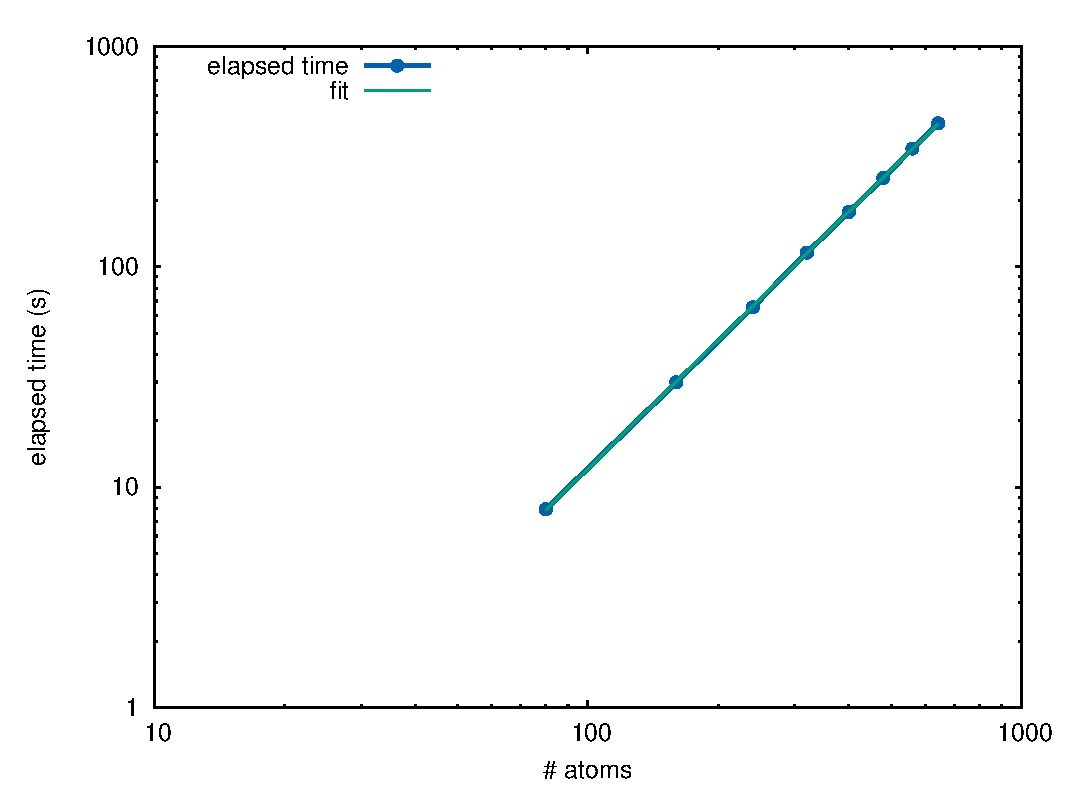
\includegraphics[width=0.6\textwidth]{figs/serial.eps}
\end{figure}

The small discrepancy between the fitted exponent in Figure \ref{fig:serial}, i.e., 1.94, and the theoretical quadratic prediction can be justified in terms of the size of the tested systems, which fall into the pre-asymptotic, rather than asymptotic region. To support this claim, we employed a second benchmark set, which included a 240 atom long chain of Crambin from the previous set, and four additional systems obtained by incrementally considering the first four chains of a larger protein (PDB reference 2QHO). We obtained systems of size ranging from 1174 to 3930 atoms. The computation of the ddPCM forces was performed using the shared-memory (OpenMP) parallel version of the code. The timings are reported in
Figure \ref{fig:para}, and the fitted, i.e., 1.99, supports our claim of asymptotic quadratic complexity. We remark that, overall, the observed timings are encouraging, despite the code not having been fully optimized. Nevertheless, the quadratic scaling makes the application of the ddPCM method to large systems challenging. 


\begin{figure}[t]
 \caption{Scaling of computation of the ddPCM forces (OpenMP parallel implementation). The results are plotted on a log-log scale, and fitted with a function of slope 1.99. The computations were performed on a dual Intel Xeon E5-2620 (v2) CPU cluster node (12 cores) equipped with 64 GB of RAM. Hyper-Threading was disabled.
\label{fig:para}}
 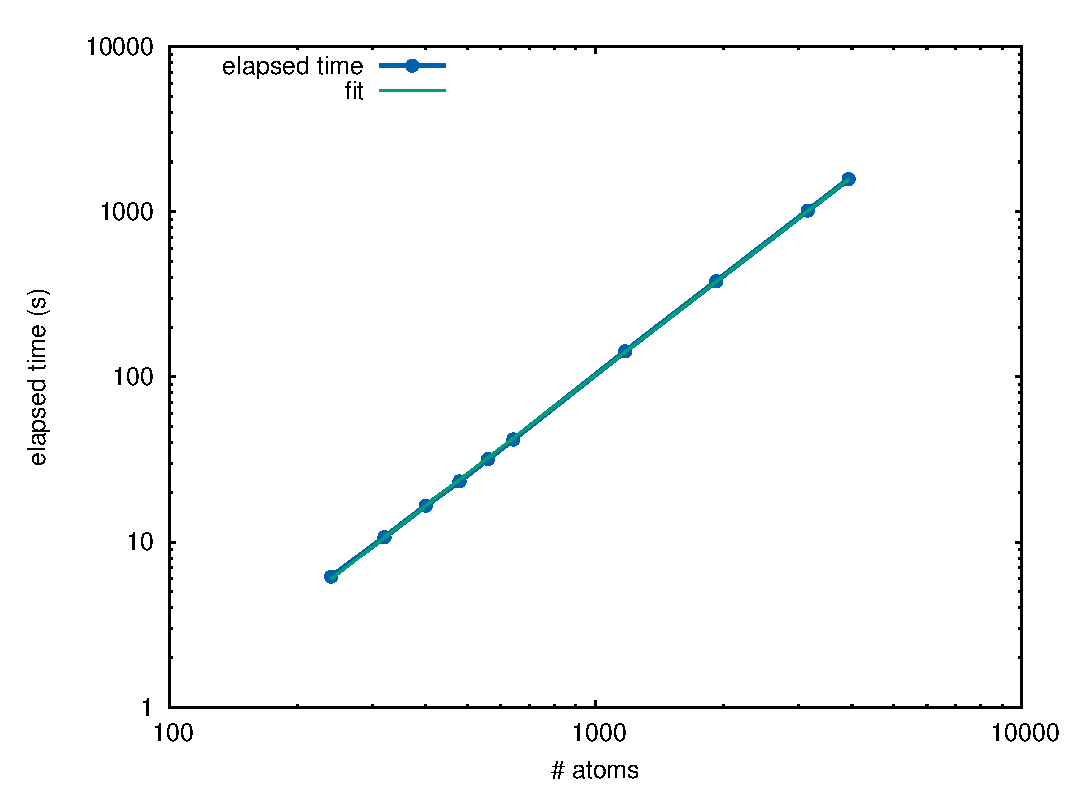
\includegraphics[width=0.6\textwidth]{figs/para.eps}
\end{figure}


